\documentclass[20pt,aspectratio=43]{beamer}
\usepackage{tikz}
\usetheme{Madrid}
\definecolor{fuzzpaint}{RGB}{255,0,255}
\definecolor{fuzzsecond}{RGB}{18,137,67}
\setbeamertemplate{navigation symbols}{}
\title{Probe}
\year=2026\month=11\day=5
\date{}
\begin{document}
\begin{frame}\begin{columns}[onlytextwidth,b]\begin{column}{0.32\textwidth}\begin{enumerate}\item<1-> Alpha has a short argument.\item<2-> 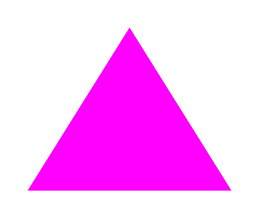
\begin{tikzpicture}[scale=1.15]\fill[fuzzpaint] (0,0)--(2.25,0)--(1.125,1.8)--cycle;\end{tikzpicture}\par Omega follows the picture.\end{enumerate}\end{column}\begin{column}{0.62\textwidth}Neighbor\end{column}\end{columns}\only<3>{}\end{frame}
\end{document}
